\subsection{reverb}
\begin{frame}{artificial reverberation}{introduction}
	\begin{itemize}
		\item	\textbf{idea}:\\
				\begin{itemize}
					\item	artificially generate the impression of envelopment and reverberation
					\item	possibly allow to modify specific characteristics of the ``modeled'' room
				\end{itemize}
		\pause
		\item	\textbf{approaches}
			\begin{itemize}
				\item	(digital) parametric reverberation (predecessors: spring, plate, room, \ldots)
				\item	fast convolution
			\end{itemize}	
	\end{itemize}
\end{frame}

\begin{frame}{artificial reverberation}{room impulse response}
	\begin{figure}
		\centerline{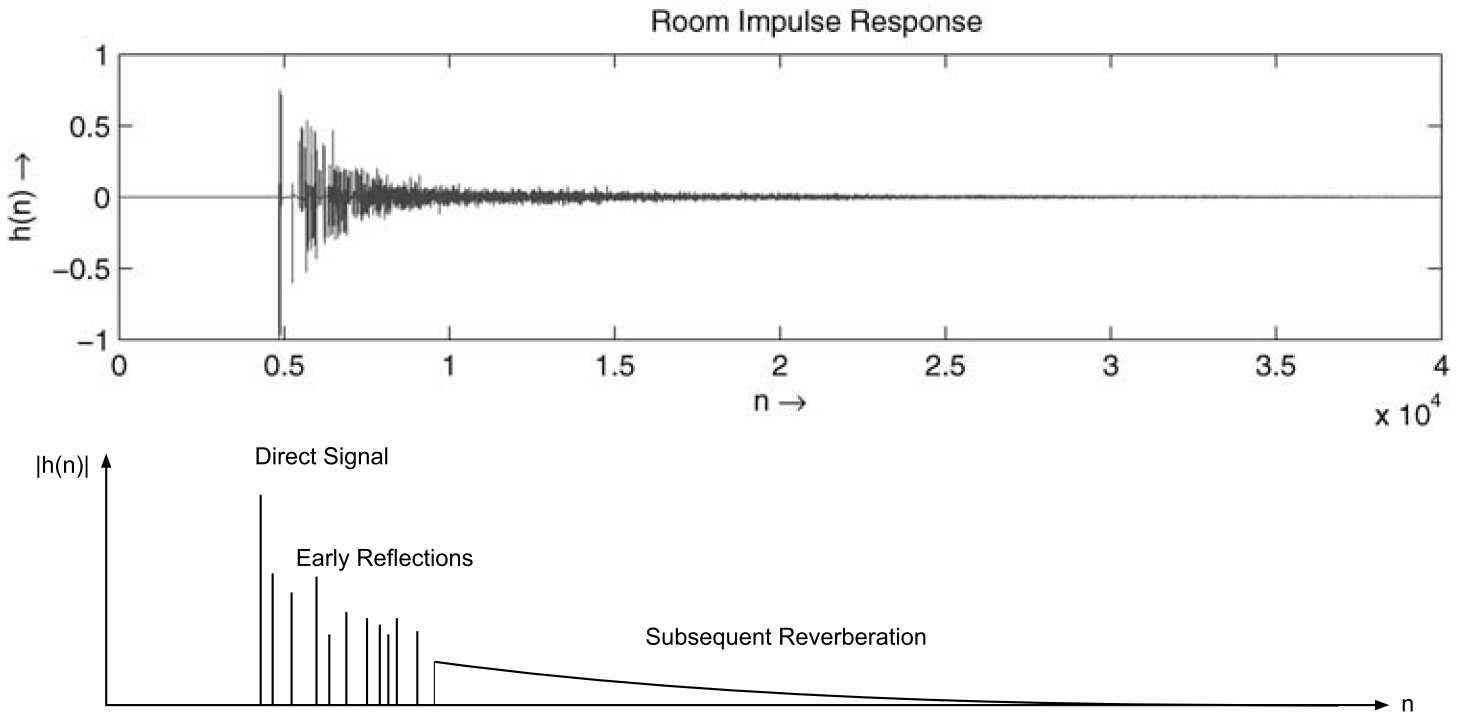
\includegraphics[scale=.4]{graph/IR}}
	\end{figure}
\end{frame}

\begin{frame}{artificial reverberation}{room impulse response: properties}
	\vspace{-5mm}
    room impulse response is sum of (filtered and delayed) reflections
	\pause
	
	\begin{itemize}
		\item	\textbf{properties}
			\begin{itemize}
				\item	level decrease is app. linear
				\item	density of reflections increases
			\end{itemize}
		\pause
        \bigskip
		\item	\textbf{description}
			\begin{itemize}
				\item	reverberation time: time in seconds for a level decrease of \unit[60]{dB}
				\item	depends mainly on
					\begin{itemize}
						\item	room \textit{volume}
						\item	surface \textit{area}
						\item	surface \textit{absorption}
					\end{itemize}
				\item	Sabine:
					\begin{equation*}
						T_\mathrm{RT} = 0.163 \unit{m^{-1}} \frac{V}{\sum{\alpha_n\cdot S_n}}
					\end{equation*}
			\end{itemize}
	\end{itemize}
\end{frame}

\begin{frame}{artificial reverberation}{traditionally used filters: comb filter}
	        \begin{figure}
				\begin{center}
	            \begin{picture}(50,30)
	
	                %boxes
	                \put(25,5){\framebox(7,6){\footnotesize{$z^{-N}$}}}
	
	                %lines horizontal
	                \put(0,20){\vector(1,0){14}}
	                \put(16,20){\vector(1,0){32}}
	                \put(50,20){\vector(1,0){5}}
	                
	                \put(15,8){\line(1,0){10}}
	                \put(42,8){\vector(-1,0){10}}
	
	                %lines vertical
	                \put(42,20){\line(0,-1){12}}
	                \put(15,8){\vector(0,1){4}}
	                \put(15,14){\vector(0,1){5}}
	                
	                %circles
	                \put(47.5,19){$\otimes$}
	                \put(13.5,19){$\oplus$} % 15-20
	                \put(13.5,12){$\otimes$}
	                
	                \put(42,20){\circle*{1}}
	
	                %text
	                \put(43,22){\footnotesize{\shortstack[c]{$b_0$}}}
	                \put(8,10){\footnotesize{\shortstack[c]{$-a_N$}}}
	
	                \put(-2,22){\footnotesize{\shortstack[c]{x(n)}}}
	                \put(52,22){\footnotesize{\shortstack[c]{y(n)}}}
	
	            \end{picture}
				\end{center}
	        \end{figure}
        	\begin{eqnarray*}
        		y(n) &=& b_0\cdot x(n) - a_N\cdot y(n-N)\\
	    		H(z) &=& \frac{b_0}{1-a_N\cdot z^{-N}}
        	\end{eqnarray*}
\end{frame}
\begin{frame}{artificial reverberation}{traditionally used filters: all pass filter}
		    \begin{figure}
				\begin{center}
		        \begin{picture}(30,40)
		
		            %boxes
		            \put(11,21){\framebox(8,8){\footnotesize{$z^{-M}$}}}
		
				
		            %lines horizontal
		            \put(0,25){\vector(1,0){11}}
		            \put(19,25){\vector(1,0){10}}
		
		            \put(31,25){\vector(1,0){4}}
		            \put(5,35){\vector(1,0){9}}
		            \put(16,35){\line(1,0){14}}
		            
		            \put(0,15){\line(1,0){14}}
		            \put(25,15){\vector(-1,0){9}}
		            \put(-5,25){\vector(1,0){4}}
		            
		            %lines vertical
		            \put(5,25){\line(0,1){10}}
		            \put(30,35){\line(0,-1){9}}
		            
		            \put(0,15){\vector(0,1){9}}
		            \put(25,25){\line(0,-1){10}}
		            
		            %circles
		            \put(13.5,34){$\otimes$} %15,35
		            \put(28.5,24){$\oplus$} % 30,25
		            \put(13.5,14){$\otimes$} % 
		            \put(-1.5,24){$\oplus$} % 0,25
		            
		            \put(5,25){\circle*{1}}
		            \put(25,25){\circle*{1}}
		
		            %text
		            \put(-5,28){\footnotesize{\shortstack[c]{x(n)}}}
		            \put(35,28){\footnotesize{\shortstack[c]{y(n)}}}
		            \put(16,36){\footnotesize{\shortstack[c]{g}}}
		            \put(16,12){\footnotesize{\shortstack[c]{-g}}}
		
		        \end{picture}
				\end{center}
		    \end{figure}
			\begin{eqnarray*}
				y(n) &=& g\cdot x(n) + x(n-M) - g\cdot y(n-M)\\
				H(z) &=& \frac{z^{-M} + g}{1 + g\cdot z^{-M}}
			\end{eqnarray*}
\end{frame}

\begin{frame}{artificial reverberation}{reverberation: Schroeder 1/2}
		\begin{figure}
			\centerline{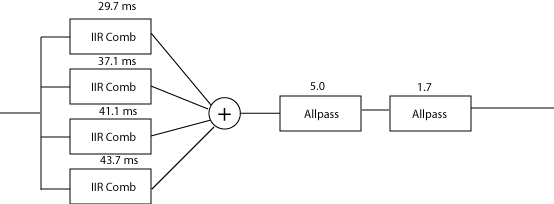
\includegraphics[scale=.5]{graph/schroeder}}
		\end{figure} 
		
		\pause
		\textbf{questions}:
		\begin{itemize}
			\item	how to change the reverberation time?
			\item	how to change the density?
		\end{itemize}
\end{frame}

\begin{frame}{artificial reverberation}{reverberation: Schroeder 2/2}
    \begin{itemize}
        \item   \textbf{problems}
            \begin{itemize}
                \item	sound coloring ($\rightarrow$ prime numbers)
                \item	periodicity
            \end{itemize}
        \pause
        \bigskip
        \item   \textbf{audio}
            \begin{itemize}
                \item   original \includeaudio{audio/sv.mp3}
                \item   wet \includeaudio{audio/svRevSchroeder.mp3}
            \end{itemize}
    \end{itemize}
\end{frame}

\begin{frame}{artificial reverberation}{reverberation: Moorer}
	\begin{itemize}
		\item	similar to Schroeder's model
		\item	more comb filters
		\item	low pass in feedback paths
		\item	simple FIR model for early reflections
        \begin{figure}
            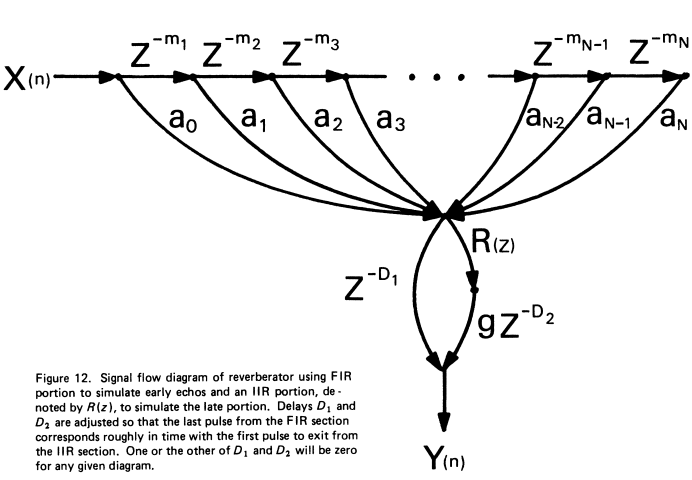
\includegraphics[scale=.3]{graph/moorer}
        \end{figure}
	\end{itemize}
    \pause
    \begin{itemize}
        \item   original \includeaudio{audio/sv.mp3}
        \item   wet \includeaudio{audio/svRevMoorer.mp3}
    \end{itemize}
\end{frame}

\begin{frame}{artificial reverberation}{other reverberation approaches: Gardner}
	\begin{figure}
		\centerline{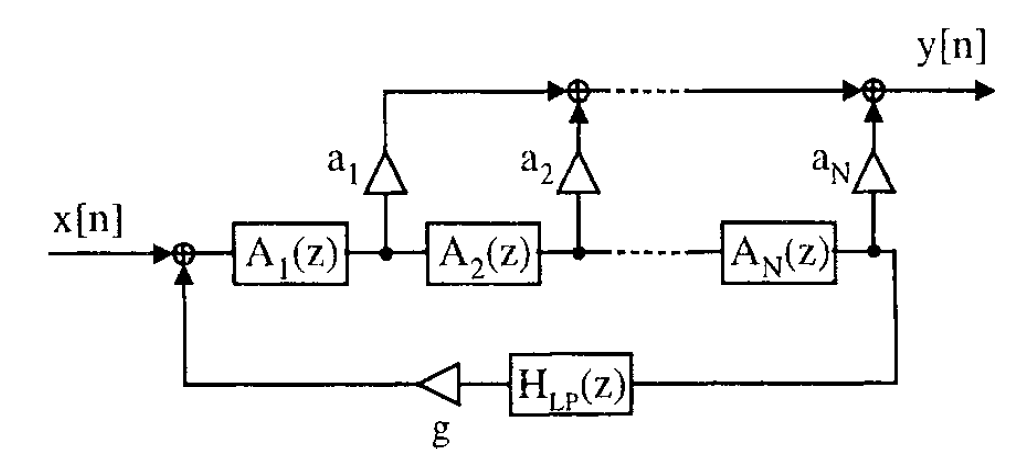
\includegraphics[scale=.4]{graph/gardnerreverb}}
	\end{figure} 
\end{frame}

\begin{frame}{artificial reverberation}{other reverberation approaches: Jot (feedback delay network)}
	\begin{figure}
		\centerline{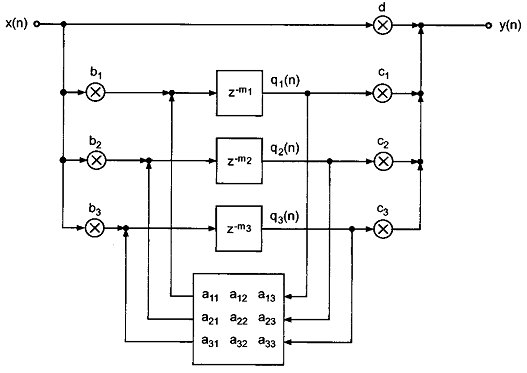
\includegraphics[scale=.5]{graph/fdn}}
	\end{figure} 
\end{frame}

\begin{frame}{artificial reverberation}{reverberation: Dattorro 1/2}
	\vspace{-7mm}
    \framezoom<1><2>[border](1.9cm,-.5cm)(6.8cm,3.5cm)
    \framezoom<1><3>[border](1.9cm,3cm)(6.8cm,4.5cm)
    \begin{figure}
		\centerline{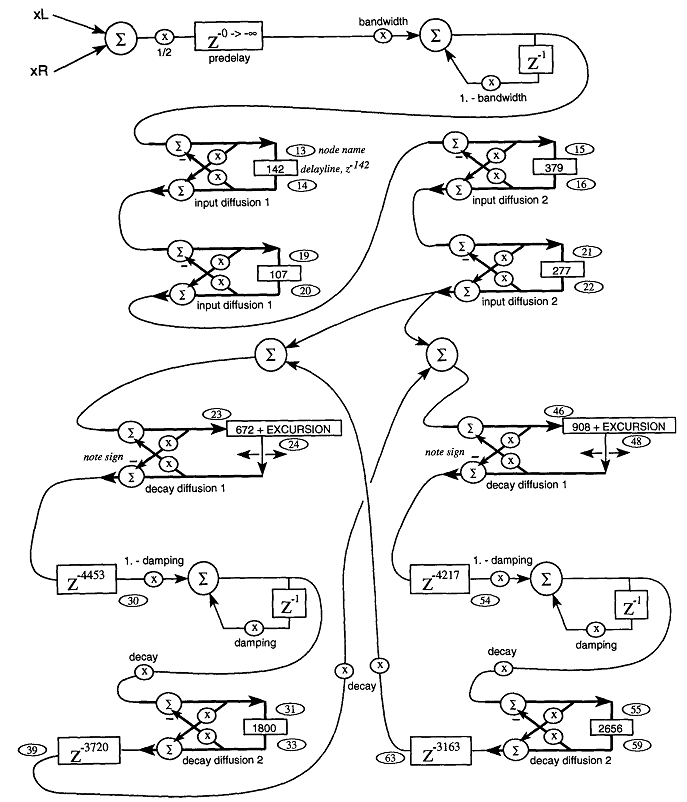
\includegraphics[scale=.37]{graph/dattorro}}
	\end{figure} 
\end{frame}

\begin{frame}{artificial reverberation}{reverberation: Dattorro 2/2}
	intention: plate reverb model \pause (dense, bright, fast build-up time)
    \bigskip
    \begin{itemize}
        \item   original \includeaudio{audio/sv.mp3}
        \item   wet (Plate) \includeaudio{audio/svRevDattorroPlate.mp3}
        \item   wet (Medium Hall) \includeaudio{audio/svRevDattorroMedHall.mp3}
        \item   wet (Cathedral) \includeaudio{audio/svRevDattorroCathed.mp3}
    \end{itemize}
\end{frame}

\begin{frame}{artificial reverberation}{early reflections: models 1/3}
	\begin{figure}
		\centerline{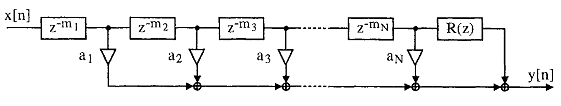
\includegraphics[scale=.6]{graph/er_simple}}
	\end{figure}
\end{frame}

\begin{frame}{artificial reverberation}{early reflections: models 2/3}
	\begin{figure}
		\centerline{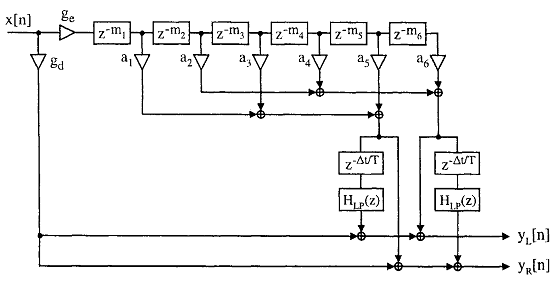
\includegraphics[scale=.6]{graph/erstandard}}
	\end{figure}
\end{frame}

\begin{frame}{artificial reverberation}{early reflections: models 3/3}
	\begin{figure}
		\centerline{\includegraphics[scale=.4]{graph/raummodell}}
	\end{figure}
\end{frame}

\begin{frame}{artificial reverberation}{quality enhancements}
	\begin{itemize}
		\item	\textbf{multi-channel processing}
			\begin{itemize}
				\item	mono in $\rightarrow$ mono out				
				\item	mono in $\rightarrow$ stereo out				
				\item	stereo in $\rightarrow$ stereo out
			\end{itemize}
		\pause
        \bigskip
		\item	\textbf{delay modulation}
			\begin{itemize}
				\item	increase ``diffusity'' and ``liveliness''
			\end{itemize}
	\end{itemize}
\end{frame}

\begin{frame}{artificial reverberation}{common parameters}
	\begin{itemize}
		\item	wetness
		\pause
		\item	reverberation time
		\pause
		\item	pre-delay
		\pause
		\item	low pass cutoff
		\pause
		\item	low pass slope
		\pause
		\item	bass boost
		\pause
		\item	ratio of early reflection/late reverberation
		\pause
		\item	diffusion, liveliness, etc.
	\end{itemize}
\end{frame}
